\subsection{Background Specifications}\label{appendix:bk}
We present the background specifications for Security Analyst, Technical Officer, Developer, and Trainer in Figure~\ref{fig:bk-sec}.
It is also easy to add more types of users by clearly defining their background specifications.

\begin{figure*}
    \centering    
{\footnotesize
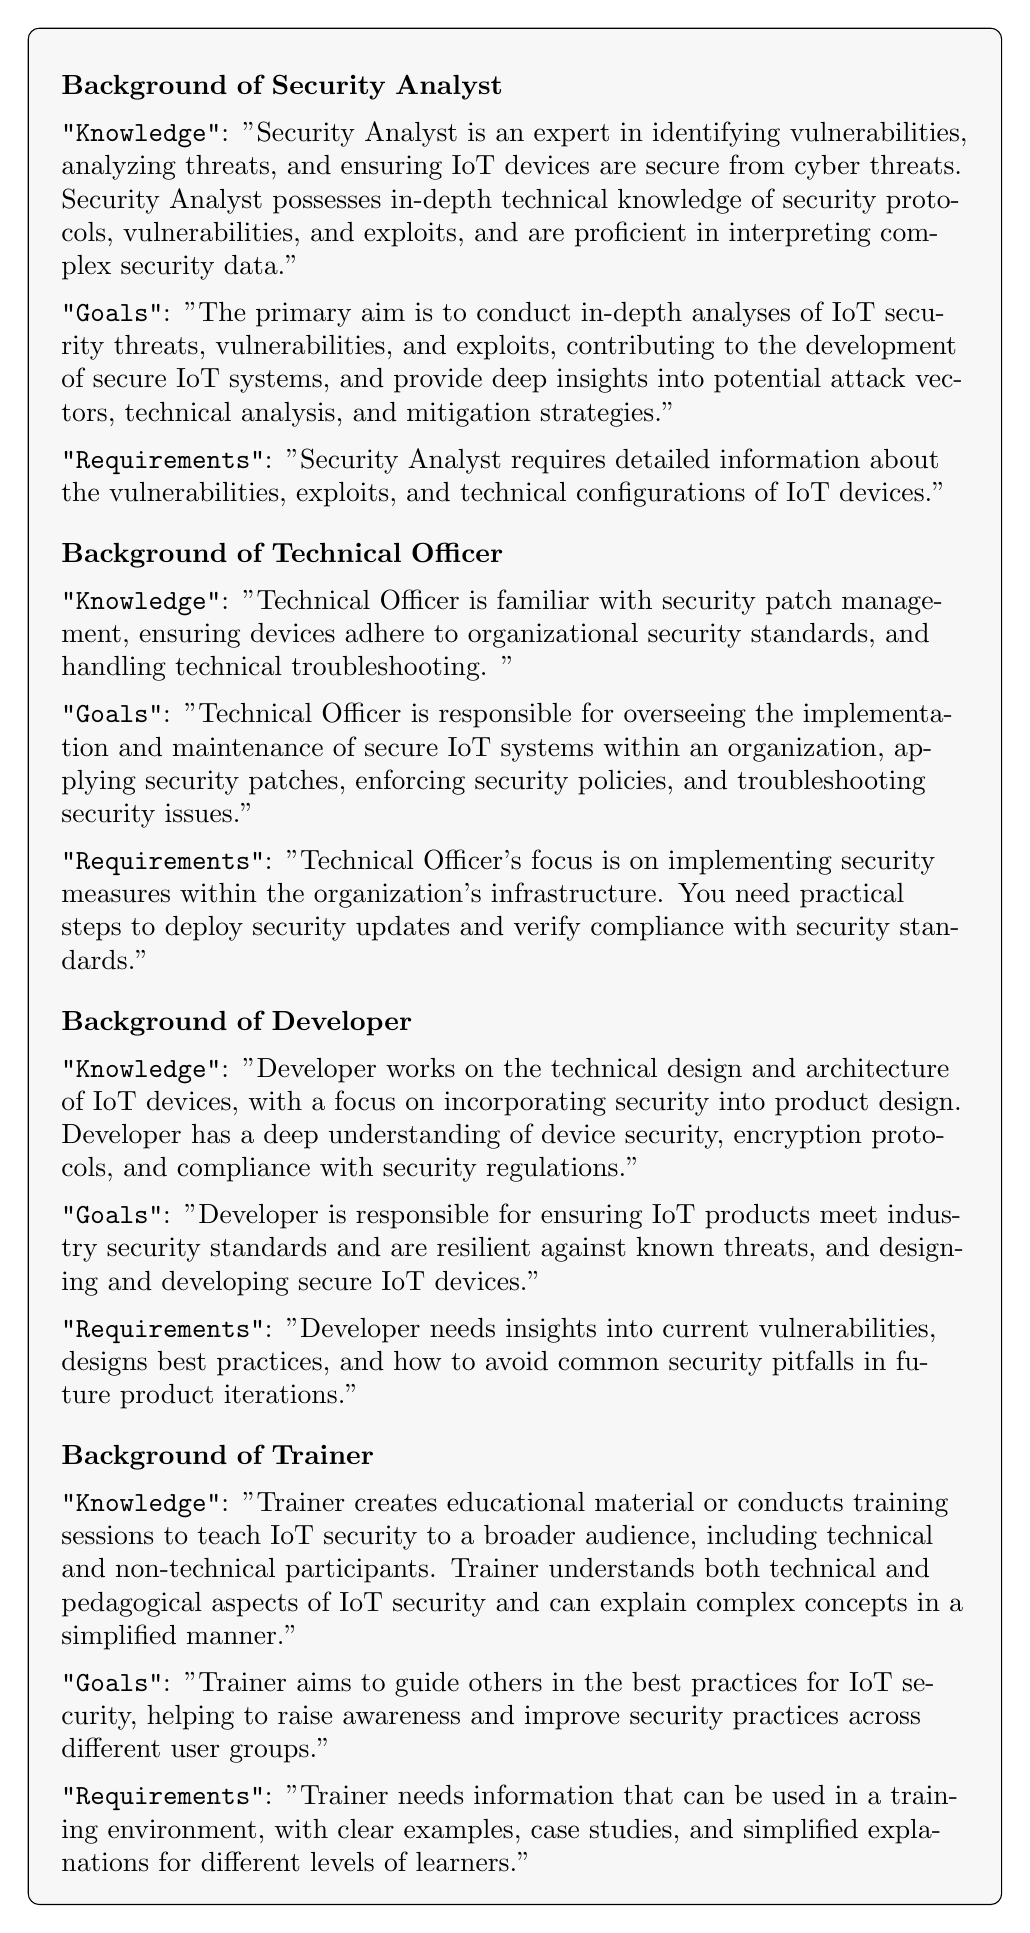
\begin{tikzpicture}
% Draw rounded rectangle with shadow
\node[rectangle, rounded corners, draw=black, fill=black!3!white, text width=0.95\textwidth, inner sep=12pt, align=left] (box) {

\textbf{Background of Security Analyst}
\vspace{5pt}\\
    \textbf{\texttt{"Knowledge"}}: "Security Analyst is an expert in identifying vulnerabilities, analyzing threats, and ensuring IoT devices are secure from cyber threats. Security Analyst possesses in-depth technical knowledge of security protocols, vulnerabilities, and exploits, and are proficient in interpreting complex security data."
    \vspace{5pt}\\
    \textbf{\texttt{"Goals"}}: "The primary aim is to conduct in-depth analyses of IoT security threats, vulnerabilities, and exploits, contributing to the development of secure IoT systems, and provide deep insights into potential attack vectors, technical analysis, and mitigation strategies."
    \vspace{5pt}\\
    \textbf{\texttt{"Requirements"}}: "Security Analyst requires detailed information about the vulnerabilities, exploits, and technical configurations of IoT devices."
\vspace{10pt}\\

\textbf{Background of Technical Officer}
\vspace{5pt}\\
\textbf{\texttt{"Knowledge"}}: "Technical Officer is familiar with security patch management, ensuring devices adhere to organizational security standards, and handling technical troubleshooting. "
\vspace{5pt}\\
\textbf{\texttt{"Goals"}}: "Technical Officer is responsible for overseeing the implementation and maintenance of secure IoT systems within an organization, applying security patches, enforcing security policies, and troubleshooting security issues."
\vspace{5pt}\\
\textbf{\texttt{"Requirements"}}: "Technical Officer's focus is on implementing security measures within the organization's infrastructure. You need practical steps to deploy security updates and verify compliance with security standards."
\vspace{10pt}\\

\textbf{Background of Developer}
\vspace{5pt}\\
\textbf{\texttt{"Knowledge"}}: "Developer works on the technical design and architecture of IoT devices, with a focus on incorporating security into product design. Developer has a deep understanding of device security, encryption protocols, and compliance with security regulations."
\vspace{5pt}\\
\textbf{\texttt{"Goals"}}: "Developer is responsible for ensuring IoT products meet industry security standards and are resilient against known threats, and designing and developing secure IoT devices."
\vspace{5pt}\\
\textbf{\texttt{"Requirements"}}: "Developer needs insights into current vulnerabilities, designs best practices, and how to avoid common security pitfalls in future product iterations."
\vspace{10pt}\\
\textbf{Background of Trainer}
\vspace{5pt}\\
\textbf{\texttt{"Knowledge"}}: "Trainer creates educational material or conducts training sessions to teach IoT security to a broader audience, including technical and non-technical participants. Trainer understands both technical and pedagogical aspects of IoT security and can explain complex concepts in a simplified manner."
\vspace{5pt}\\
\textbf{\texttt{"Goals"}}: "Trainer aims to guide others in the best practices for IoT security, helping to raise awareness and improve security practices across different user groups."
\vspace{5pt}\\
\textbf{\texttt{"Requirements"}}: "Trainer needs information that can be used in a training environment, with clear examples, case studies, and simplified explanations for different levels of learners."
};
\end{tikzpicture}
}
\caption{The background specifications for Security Analyst, Technical Officer, Developer, and Trainer, utilized to guide the \chatiot\ to generate answers.}
\label{fig:bk-sec}
\end{figure*}

\iffalse

\begin{figure*}
    \centering    
{\footnotesize
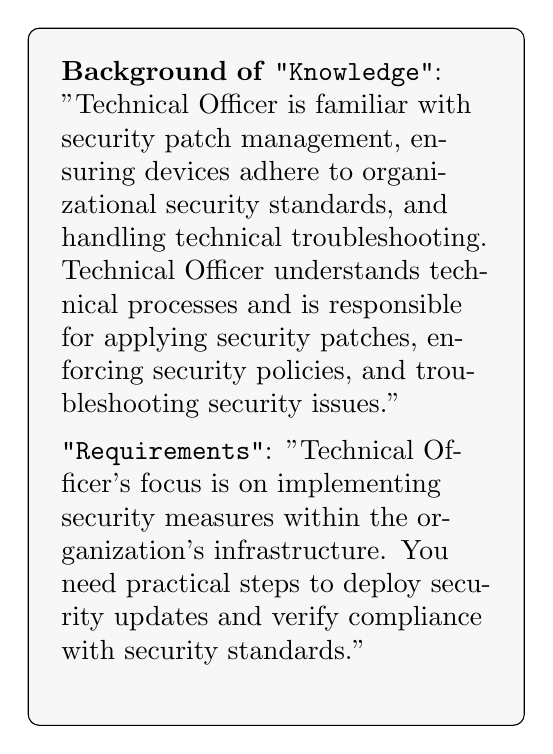
\begin{tikzpicture}
% Draw rounded rectangle with shadow
\node[rectangle, rounded corners, draw=black, fill=black!3!white, text width=0.45\textwidth, inner sep=12pt, align=left] (box) {
\textbf{Background of}
    \textbf{\texttt{"Knowledge"}}: "Technical Officer is familiar with security patch management, ensuring devices adhere to organizational security standards, and handling technical troubleshooting. Technical Officer understands technical processes and is responsible for applying security patches, enforcing security policies, and troubleshooting security issues."
    \vspace{5pt}\\
    \textbf{\texttt{"Requirements"}}: "Technical Officer's focus is on implementing security measures within the organization's infrastructure. You need practical steps to deploy security updates and verify compliance with security standards."
\vspace{10pt}\\


};
\end{tikzpicture}
}
\caption{The specific background for technical officer utilized to guide the \chatiot\ to generate Technical Officer-friendly outputs.}
\label{fig:bk-techofficer}
\end{figure*}

\begin{figure}
    \centering    
{\footnotesize
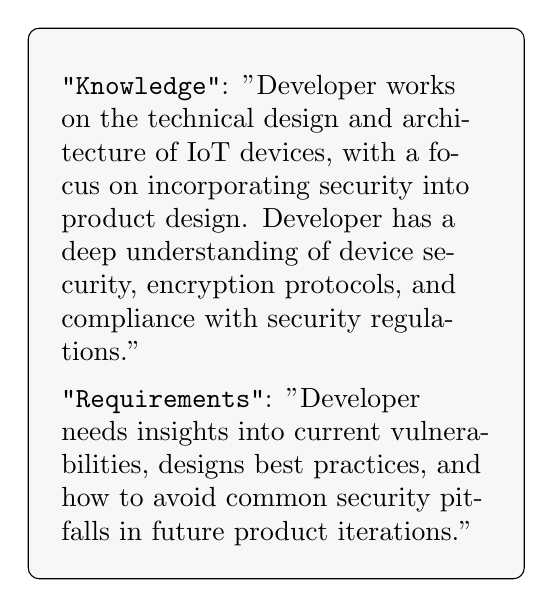
\begin{tikzpicture}
% Draw rounded rectangle with shadow
\node[rectangle, rounded corners, draw=black, fill=black!3!white, text width=0.45\textwidth, inner sep=12pt, align=left] (box) {

    \textbf{\texttt{"Knowledge"}}: "Developer works on the technical design and architecture of IoT devices, with a focus on incorporating security into product design. Developer has a deep understanding of device security, encryption protocols, and compliance with security regulations."
    \vspace{5pt}\\
    \textbf{\texttt{"Requirements"}}: "Developer needs insights into current vulnerabilities, designs best practices, and how to avoid common security pitfalls in future product iterations."
};
\end{tikzpicture}
}
\caption{The specific background for developer utilized to guide the \chatiot\ to generate Developer-friendly outputs.}
\label{fig:bk-dev}
\end{figure}

\begin{figure}
    \centering    
{\footnotesize
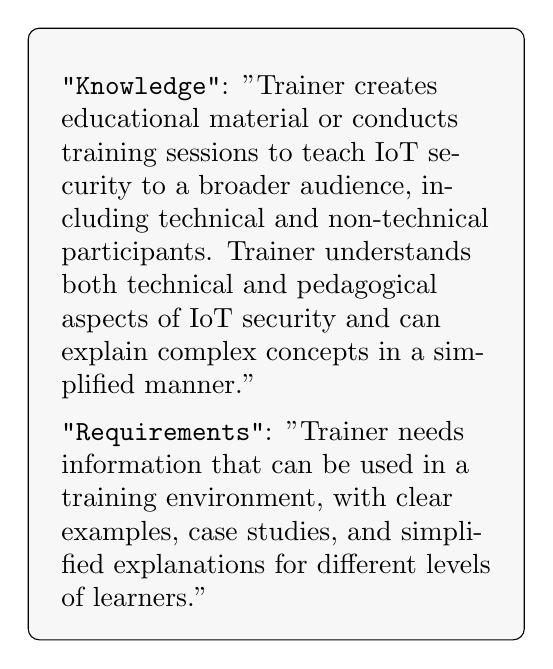
\begin{tikzpicture}
% Draw rounded rectangle with shadow
\node[rectangle, rounded corners, draw=black, fill=black!3!white, text width=0.45\textwidth, inner sep=12pt, align=left] (box) {

    \textbf{\texttt{"Knowledge"}}: "Trainer creates educational material or conducts training sessions to teach IoT security to a broader audience, including technical and non-technical participants. Trainer understands both technical and pedagogical aspects of IoT security and can explain complex concepts in a simplified manner."
    \vspace{5pt}\\
    \textbf{\texttt{"Requirements"}}: "Trainer needs information that can be used in a training environment, with clear examples, case studies, and simplified explanations for different levels of learners."
};
\end{tikzpicture}
}
\caption{The specific background for consumer utilized to guide the \chatiot\ to generate Trainer-friendly outputs.}
\label{fig:bk-trainer}
\end{figure}
\fi